\section{Bayesian active learning by disagreement\label{sec:active}}

The goal of active learning is to choose item pairs such that we learn the
preference functions for the users using minimal data.
Information theoretic approaches to active learning are popular because
they do not require prior knowledge of loss functions or test domains.
The central goal is to identify the new data point that maximizes the expected reduction in
posterior entropy. For preference learning
(see Section \ref{sec:prefKernel}), this implies
choosing the new item features $\mathbf{x}_i$ and $\mathbf{x}_j$ that maximize

\vspace{-0.65cm}
{\small
\begin{align}   
\ent[\mathcal{P}(g|\mathcal{D})] - \E_{\mathcal{P}(y|\mathbf{x}_i,\mathbf{x}_j,\data)} \left[ \ent[\mathcal{P}(g|y,\mathbf{x}_i,\mathbf{x}_j,\data)]\right]\,,
\label{eqn:ent_change}
\end{align}
}

\vspace{-0.65cm}
\normalsize where $\mathcal{D}$ are the user preferences observed so far and
$\ent[p(x)]=-\int p(x)\log p(x)\,dx$ represents the Shannon entropy. 
This framework, originally proposed in \cite{lindley1956},
is difficult to apply directly to models based on GPs.
In these models, entropies can be poorly
defined or their computation can be intractable.
In practice, current approaches make
approximations for the computation of the posterior entropy \cite{mackay1992,lawrence2002}. 
However, a second difficulty arises; if $n$ new data points are
available for selection, with $|\{-1,1\}|=2$ possible values for $y$.
Then $\mathcal{O}(2n)$ potentially expensive posterior updates are required to find the maximizer
of (\ref{eqn:ent_change}): one for every available feature vector and possible class value.
This is often too expensive in practice.

A solution consists in noting that (\ref{eqn:ent_change}) is equivalent to the conditioned mutual information between $y$ and $g$.
Using this we can rearrange this equation to compute entropies in $\y$ space:

\vspace{-0.65cm}
{\small
\begin{align}
\ent[\mathcal{P}(y|\mathbf{x}_i,\mathbf{x}_j,\data)] - \E_{\mathcal{P}(g|\data)}
\left[\ent\left[ \mathcal{P}(y|\mathbf{x}_i,\mathbf{x}_j,g)\right]\right]\,. \label{eqn:rearrangement} 
\end{align}
}

\vspace{-0.65cm}
\normalsize This overcomes the previous challenges. Entropies are now evaluated in
output space, which has low dimension. Furthermore, $g$ is now conditioned only upon $\data$,
so only $\mathcal{O}(1)$ updates of the posterior distribution are required. 
We only need to recompute the posterior once per data point selected, not for every possible data point under consideration.
Expression (\ref{eqn:rearrangement}) also provides us with an intuition about the objective;
we seek the $\mathbf{x}_i$ and $\mathbf{x}_j$ for which a) the model is marginally
uncertain about $y$ (high $\ent[\mathcal{P}(\y | \mathbf{x}_i,\mathbf{x}_j, \data)]$) and
b) conditioned on a particular value of $g$ the model is confident about $y$
(low $\E_{\mathcal{P}(g|\data)} \left[\ent [ \mathcal{P}(y |\mathbf{x}_i,\mathbf{x}_j,g] \right)]$).
This can be interpreted as seeking the pair $\mathbf{x}_i$ and $\mathbf{x}_j$ for which the latent functions $g$, under the posterior, `disagree' with each other the most about the outcome, that is, the preference judgement.
Therefore, we refer to this objective as Bayesian Active Learning by Disagreement (BALD).
This method is independent of the approach used for inference, something which does not hold for
the techniques described in \cite{mackay1992, krishnapuram2004, lawrence2002}. 
In the following section we show how (\ref{eqn:rearrangement}) can be applied to binary classification with GPs, and hence via the preference kernel also to any preference learning problem.


\subsection{BALD in binary classification with GPs}

\begin{SCfigure}
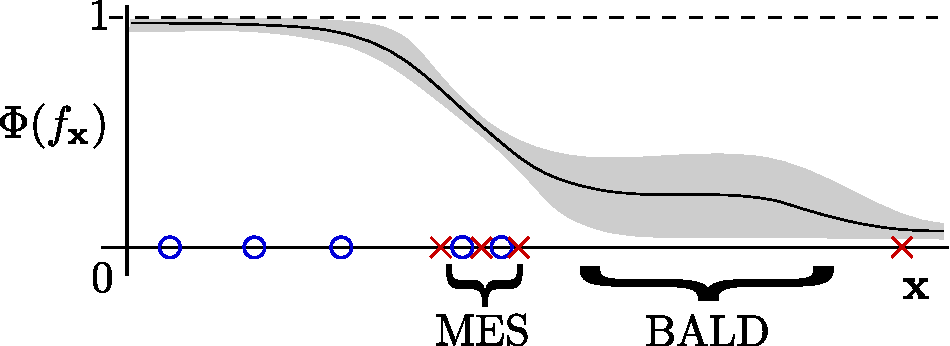
\includegraphics[scale = 0.45]{figs/BALD_eg.pdf}
\caption{Toy example with 1D input. Circles and crosses
denote labelled data. The plot shows the mean and variance of the GP predictive
distribution. Maximum Entropy Sampling (MES)
samples from the region of highest marginal uncertainty, ignoring the
second term in \eqref{eqn:rearrangement}. BALD samples 
from the region of greatest uncertainty in the latent function.\label{fig:BALD}}
\end{SCfigure}

Most approximate inference methods for the problem of binary classification with
GPs produce a Gaussian approximation to the posterior distribution of $f$, the
latent function of interest. In the binary GP classifier, the entropy of $y$ given the corresponding value of $f$ 
can be expressed in terms of the binary entropy function, $\mathrm{h}[f]=- f\log f - (1-f)\log(1-f)$.
In particular,
$\ent[p(y\vert\x,\latfun)] = \mathrm{h}\left[\Phi(\latfun(\x)\right]$.
When a Gaussian is used to approximate the posterior of $f$,  we have that
for each $\x$, $\latfun_{\x} = \latfun(\x)$ will follow a Gaussian distribution with mean $\mu_{\x}$ and
variance $\sigma_{\x}^2$.
The first term in (\ref{eqn:rearrangement}), that is, $\ent[p(y\vert\x,\data)]$, can be handled analytically in this case:
$\ent[p(y\vert\x,\data)] \approx \mathrm{h}\left[ \int \Phi( \latfun_{\x} )
\mathcal{N}(\latfun_{\x}| \mu_{\x},\sigma_{\x}^2) d\latfun_{\x} \right]
= \mathrm{h} \left[ \Phi\left( \mu_{\x} (\sigma^2_{\x} + 1)^{-1/2}\right)\right]$,
where $\approx$ represents here the Gaussian approximation to the posterior of $\latfun_{\x}$.
The second term in (\ref{eqn:rearrangement}), that is,
$\E_{p(\latfun\vert\data)} \left[ \ent[p(\y\vert\x, \latfun)] \right]$, can be approximated as
$ \E_{p(f\vert\data)} \left[ \ent[p(\y\vert\x, \latfun)] \right] \approx
C(\sigma_{\x}^2 + C^2)^{-1/2}\exp\left(-\mu_{\x}^2(2\left(\sigma_{\x}^2 + C^2\right))^{-1}\right)$,
where $C=\sqrt{\pi\log 2 / 2}$. This result is obtained by
using the Gaussian approximation to the posterior of $\latfun_{\x}$
and then approximating $\mathrm{h}[\Phi(\latfun_{\x})]$
by the squared exponential curve $\exp(-\latfun_{\x}^2/\pi\log 2)$
(details can be found in Section 3 of the supplementary material).

To summarize, the BALD algorithm for active binary GP classification / preference learning first applies
any approximate inference method to obtain the posterior mean
$\mu_{\x}$ and variance $\sigma_{\x}^2$ of $f$ at each point of interest $\x$. Then, it selects the
feature vector $\x$ that maximizes the objective

\vspace{-0.5cm}
{\small
\begin{equation}
\mathrm{h} \left[ \Phi\left( \mu_{\x}(\sigma^2_{\x} + 1)^{-1/2} \right)\right] -
C(\sigma_{\x}^2 + C^2)^{-1/2} \exp\left(-\mu_{\x}^2(2\left(\sigma_{\x}^2 + C^2\right))^{-1}\right)\,.\label{eqn:BALD}
\end{equation}
}

\vspace{-0.6cm}
\normalsize BALD assigns a high value to the feature vector $\x$ when the model is both uncertain
about the label ($\mu_{\x}$ close to 0) and there is high uncertainty about $f_\x$
($\sigma_{\x}^2$ is large). The second term prevents BALD from sampling in regions
where the model knows that the label is uncertain. Figure \ref{fig:BALD} illustrates
the differences between BALD and Maximum Entropy Sampling \cite{sebastiani2000} (details in the supplementary material, Section 5).
MES considers only marginal uncertainty (the first term in \eqref{eqn:BALD}), and hence seeks data in an
uninformative region of the plot. By contrast, BALD samples data from the
region of greatest uncertainty in the latent function.
